\documentclass[a4paper,14pt]{extarticle}

\usepackage{indentfirst}
\usepackage[utf8]{inputenc}
\usepackage[T1]{fontenc}
\usepackage[utf8]{vietnam}
\usepackage{float}
\usepackage{hyperref}

\usepackage{tikz}
\usepackage{gensymb}

\usepackage{enumitem}
\setitemize{itemsep=1pt}
\setlist{nolistsep}

\usepackage{times}
\usepackage{geometry}
\geometry{
	a4paper,
	% total={170mm,257mm},
	left=30mm,
	right=20mm,
	top=20mm,
	bottom=20mm,
}

% ============ Document starts here =====================================================

\title{\textbf{Nhận diện một số sâu bệnh\\thường gặp trên cây cà phê\\qua hình thái của lá}}
\author{Nguyễn Quang Trường\\12 Toán - Trường THPT Chuyên Nguyễn Tất Thành}
\date{Kon Tum, ngày 15 tháng 12 năn 2021}

\begin{document}
\tableofcontents
\pagebreak

\centerline{\textbf{DỰ ÁN:}}

\begingroup
	\fontsize{18pt}{1pt}\selectfont
	\centerline{\textbf{NHẬN DIỆN MỘT SỐ SÂU BỆNH THƯỜNG GẶP}}
	\centerline{\textbf{TRÊN CÂY CÀ PHÊ QUA HÌNH THÁI CỦA LÁ}}
\endgroup

\section{Lý do chọn đề tài}
Kon Tum là một tỉnh thuộc khu vực Tây Nguyên, nổi tiếng với những loài cây công nghiệp lâu năm. Trong đó, cà phê có vai trò quan trọng đối với người dân nơi đây, đặc biệt là với đồng bào dân tộc thiểu số, giúp xóa đói, giảm nghèo, mang lại nguồn thu nhập lớn cho người dân tỉnh nhà.

Tuy nhiên, hằng năm, sâu bệnh trên cây cà phê đã gây thiệt hại nặng nề cho bà con và các doanh nghiệp sản xuất, chế biến cà phê.

Vì vậy, dự án: \textbf{Nhận diện một số sâu bệnh thường gặp trên cây cà phê qua hình thái của lá} đã được nghiên cứu và phát triển. Đây là một hệ thống nhận diện thông minh, tương đối chính xác, nhằm giúp người dân, nhất là đồng bào dân tộc thiểu số nhận diện một số sâu bệnh thường gặp trên cây cà phê dễ dàng, thuận tiện để có các biện pháp phòng trừ sâu bệnh hiệu quả, góp phần cải thiện ngành trồng trọt cây cà phê tại tỉnh Kon Tum.

\section{Tìm hiểu vấn đề}

	\subsection{Câu hỏi nghiên cứu}
	Trước khi nghiên cứu, một số câu hỏi nghiên cứu được đưa ra như sau:
	\begin{itemize}
		\item Hiện tại, có những phương pháp nào để chẩn đoán sâu bệnh trên
		cây cà phê?
		\item Máy tính có thể chẩn đoán được không? Làm thế nào để chẩn đoán mà không cần đòi hỏi kiến thức chuyên sâu từ con người?
	\end{itemize}

		\subsubsection{Một số phương pháp hiện tại}
		Theo tìm hiểu của tác giả, hiện nay có hai phương pháp chính để chẩn đoán sâu bệnh.
		
		Phương pháp đầu tiên: chẩn đoán thông qua đặc điểm hình thái trên lá. Ưu điểm là nhanh chóng, thuận tiện, chi phí thấp... Tuy nhiên, nhược điểm rõ ràng nhất là khó phát hiện được các sâu bệnh phức tạp, ít thể hiện trên hình thái mà phải phân tích chuyên sâu.
		
		Phương pháp thứ hai: phân tích cấu trúc lá trong phòng thí nghiệm. Phương pháp này cho độ chính xác cao hơn, xác định được những sâu bệnh phức tạp hơn mà không thể quan sát bằng mắt thường. Nhưng việc nghiên cứu trong phòng thí nghiệm đòi hỏi nhiều thời gian, công sức để phân tích, chi phí cho cơ sở vật chất...
		
		Với mong muốn xây dựng một giải pháp nhanh chóng và thuận tiện, phương pháp nghiên cứu thông qua đặc điểm hình thái là phương pháp được lựa chọn làm cơ sở cho việc xây dựng giải pháp.

		\subsubsection{Mục tiêu dự án}
		Dự án nghiên cứu nhằm:
		\begin{itemize}
			\item Xây dựng một hệ thống giúp người dân, đặc biệt là đồng bào dân tộc thiểu số (đa số có trình độ dân trí thấp, chưa biết ứng dụng khoa học kĩ thuật vào canh tác) nhận diện các loại sâu bệnh trên cây cà phê qua hình ảnh với độ chính xác cao;
			\item Ứng dụng hệ thống vào thực tiễn tại địa phương, giúp giảm thiểu thiệt hại do sâu bệnh gây ra, góp phần phát triển kinh tế - xã hội trên địa bàn, giúp đồng bào dân tộc thiểu số vươn lên thoát nghèo, làm giàu trên chính quê hương của mình.
		\end{itemize}
			
	\subsection{Ý nghĩa của dự án}
		\subsubsection{Ý nghĩa khoa học}
		Đề tài nghiên cứu phương pháp nhận diện qua hình ảnh, tuy phổ biến trên những đối tượng khác nhưng lại ít được quan tâm trên cây cà phê. Vì vậy, tác giả mong muốn đề tài này sẽ mở rộng nghiên cứu nhận diện hình ảnh trên cây cà phê trong tương lai.

		\subsubsection{Ý nghĩa xã hội}
		Đối tượng nghiên cứu của dự án là cây cà phê, một trong những cây công nghiệp quan trọng ở tỉnh Kon Tum. Do đó, thông qua việc nghiên cứu dự án, tác giả muốn giúp người dân, đặc biệt là đồng bào dân tộc thiểu số dễ dàng nhận diện một số sâu bệnh cơ bản để có cách phòng trừ hiệu quả, góp phần xóa đói, giảm nghèo, phát triển kinh tế - xã hội trên địa bàn.

\section{Nghiên cứu chính}
	\subsection{Kế hoạch và quy trình}
	\subsubsection{Kế hoạch nghiên cứu}

	\begin{figure}[H]
		\centering
		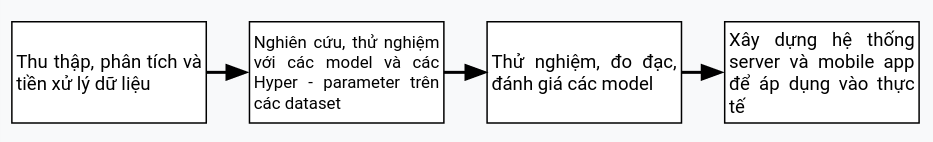
\includegraphics[scale=0.6]{images/plans.png}
		\caption{Kế hoạch nghiên cứu}
	\end{figure}

	\subsubsection{Quy trình hoạt động}
	\begin{figure}[H]
		\centering
		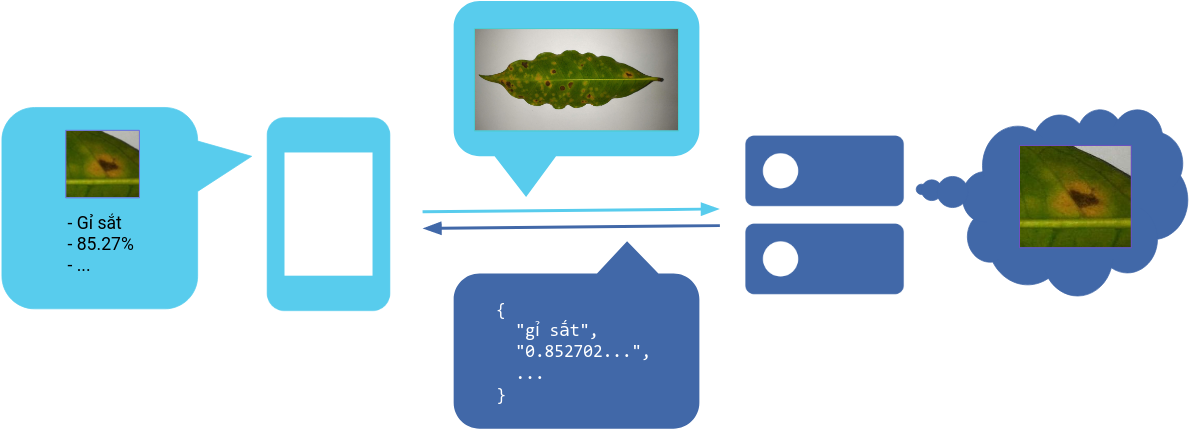
\includegraphics[scale=0.4]{images/chart.png}
		\caption{Thiết kế quy trình hoạt động}
	\end{figure}

	\subsection{Dữ liệu}
	Dữ liệu được kết hợp thu thập từ thực địa và từ các dataset khác trên mạng. Dữ liệu từ thực địa được thu thập tại các xã, thị trấn thuộc huyện Đăk Hà và xã Ia Chim, thành phố Kon Tum, tỉnh Kon Tum. Mẫu vật được đặt trên nền trắng, dưới điều kiện kiểm soát một phần.

	Một dataset gồm 1685 bức ảnh chụp các lá cà phê (bao gồm lá bình thường và lá sâu bệnh) đã được thu thập và phân loại. Kích thước của mỗi ảnh là 2048 x 1024.

	\begin{figure}[H]
		\centering
		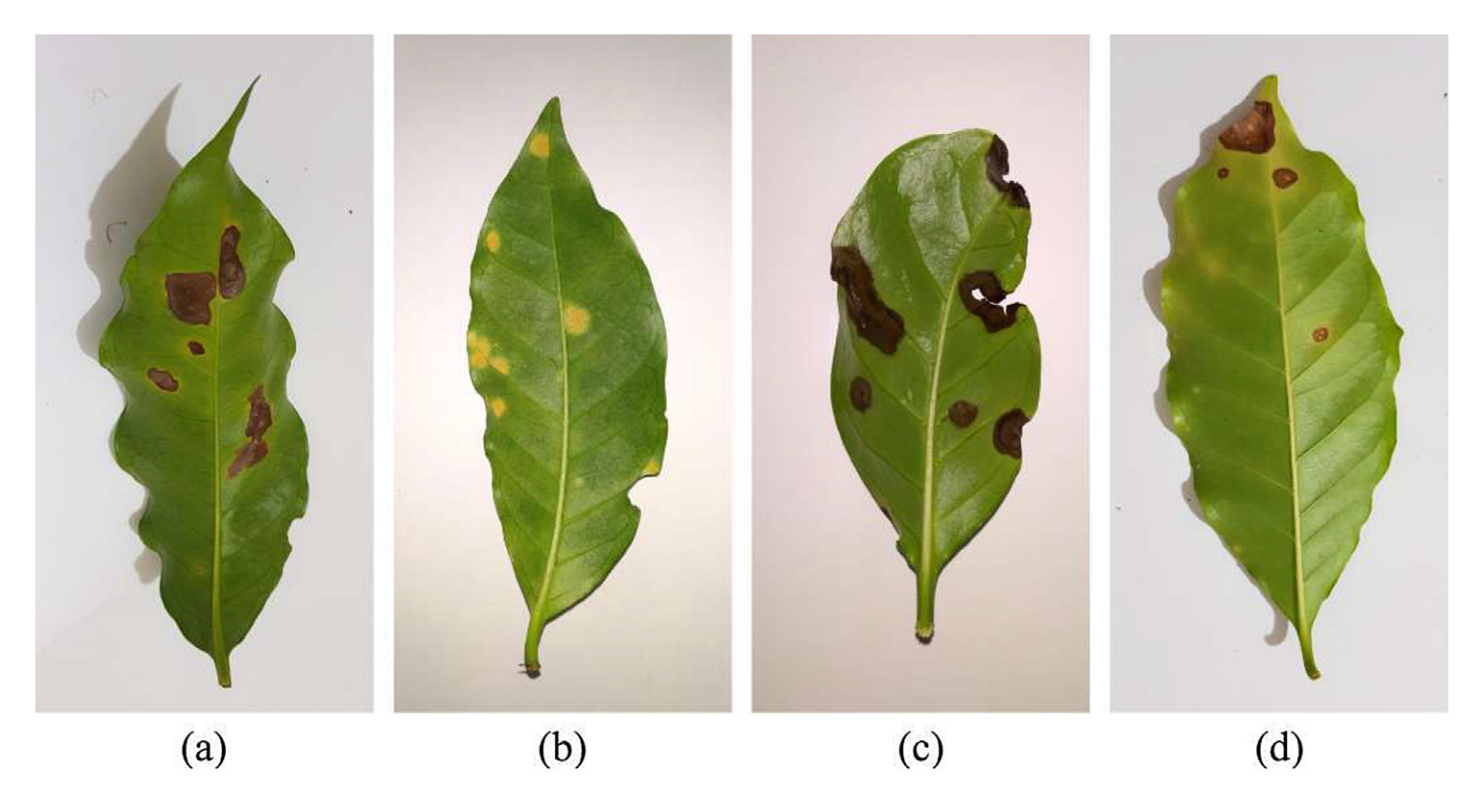
\includegraphics[scale=0.35]{images/image1}
		\caption{Sâu vẽ bùa (a), Gỉ sắt (b), Đốm nâu (c), Đốm mắt cua (d)}
	\end{figure}

	\begin{figure}[H]
		\centering
		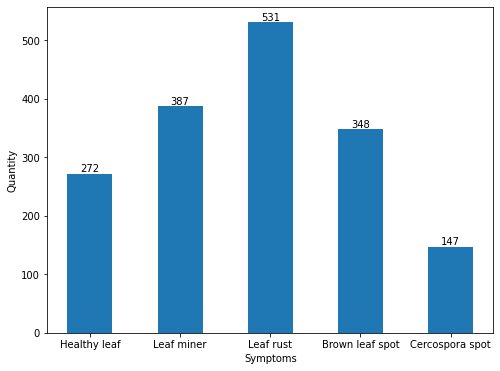
\includegraphics[scale=0.6]{images/original_dataset}
		\caption{Thống kê dữ liệu thu thập được}
	\end{figure}

	Tuy nhiên, mỗi bức ảnh có kích thước rất lớn, gây khó khăn trong quá trình xử lý về sau. Do đó, những vùng có sâu bệnh sẽ được cắt ra. Những vùng hoàn toàn bình thường trên lá cũng sẽ được cắt, nhằm mục đích đối chiếu với các vùng sâu bệnh. Sau tiền xử lý, thu được 2722 bức ảnh cắt xung quanh vùng có sâu bệnh và không có sâu bệnh trên lá. Kích thước của mỗi ảnh là 224 x 224.

	\begin{figure}[H]
		\centering
		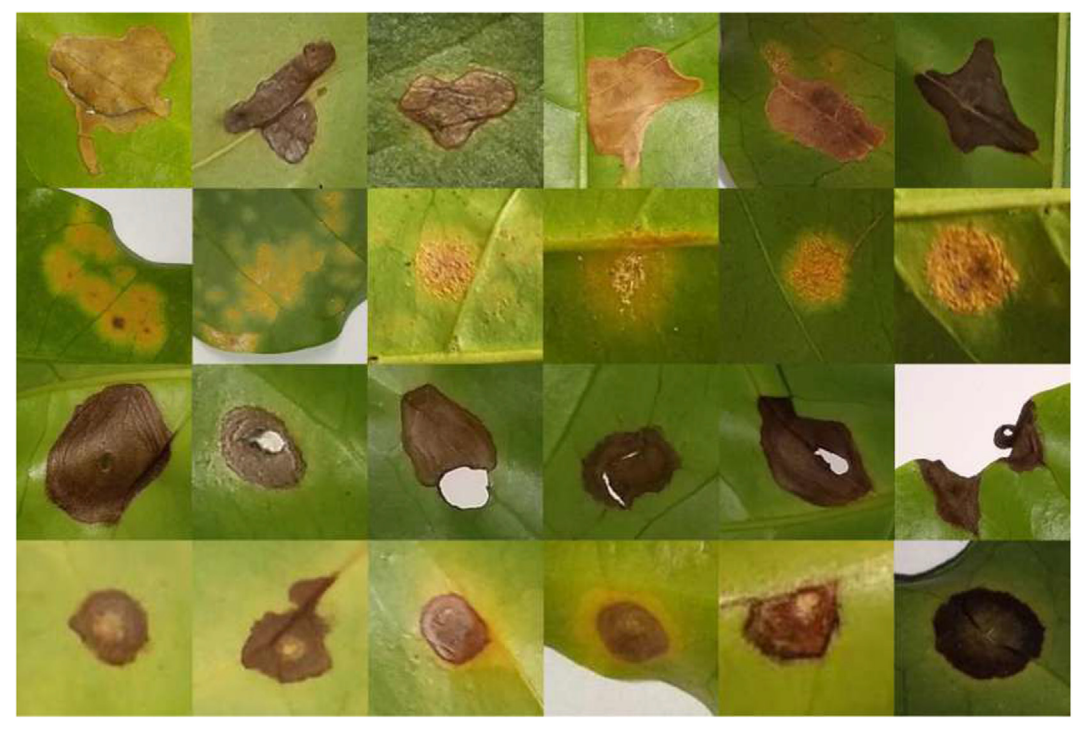
\includegraphics[scale=0.3]{images/image3}
		\caption{Các vùng được cắt sau tiền xử lý}
	\end{figure}
	
	\begin{figure}[H]
		\centering
		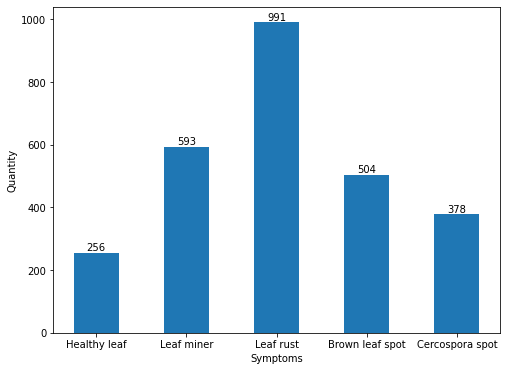
\includegraphics[scale=0.6]{images/processed_dataset}
		\caption{Thống kê dữ liệu sau tiền xử lý}
	\end{figure}

	Như vậy, có hai dataset: dataset gốc (gồm các ảnh chưa xử lý) và dataset đã qua xử lý. Từng dataset được chia ra thành training set, validation set và test set, theo tỉ lệ 70-15-15. Data Augmentation được áp dụng trên các tập để tăng cường và cân bằng dữ liệu cho các set.

	\begin{table}[H]
		\centering
		\renewcommand{\arraystretch}{1.2}
		\begin{tabular}{|c|c|}
		\hline
		Cấu hình         & Giá trị         \\ \hline
		Rescaling factor & $\frac{1}{255}$ \\ \hline
		Rotation range   & 180$\degree$    \\ \hline
		Sheer range      & 20\%            \\ \hline
		Zoom range       & 20\%            \\ \hline
		Random flip      & true            \\ \hline
		\end{tabular}

		\caption{Cấu hình Data Augmentation}
	\end{table}

	\begin{figure}[H]
		\centering
		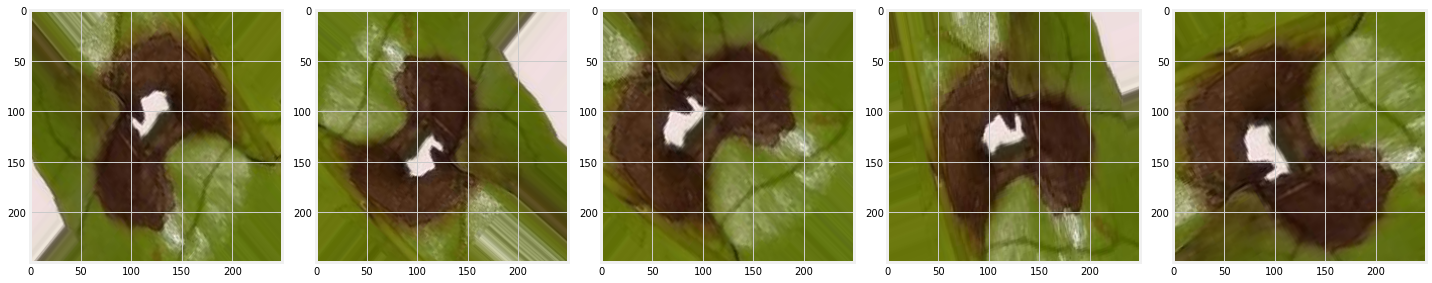
\includegraphics[scale=0.25]{images/image2}
		\caption{Ảnh được chỉnh sửa qua Data Augmentation}
	\end{figure}

	\subsection{Mô hình}
	Machine Learning đang được ứng dụng rộng rãi, hỗ trợ rất nhiều lĩnh vực trong đời sống. Machine Learning có khả năng học từ data, và ứng dụng những gì học được để giải quyết các bài toán cụ thể.

	Deep Learning, một nhánh của Machine Learning, mô phỏng cách não bộ con người tiếp nhận và xử lý thông tin bằng một neural network gồm nhiều tầng xếp lên nhau. Deep Learning có khả năng tự chiết xuất đặc tính từ data, và càng nhiều data thì model Deep Learning càng hiệu quả. Deep Learning thường là giải pháp cho các bài toán phân loại hình ảnh.

	Các model được thử nghiệm trong dự án là các Deep Learning model, bao gồm: InceptionV3, MobileNetV2, ResNet50V2, VGG16 và Xception. Những model này đều đã được học qua ImageNet và được tiếp tục luyện trên toàn bộ mạng bằng data mới mà không đóng băng thông số nào.

	\begin{table}[H]
		\centering
		\begin{tabular}{|c|c|c|}
		\hline
		Kiến trúc   & Số lượng tham số (triệu) & Số tầng \\ \hline
		InceptionV3 & 24                       & 48      \\
		MobileNetV2 & 2,2                      & 54      \\
		ResNet50V2  & 25                       & 50      \\
		VGG16       & 138                      & 16      \\
		Xception    & 23                       & 71      \\ \hline
		\end{tabular}

		\caption{Thông số của các kiến trúc được thử nghiệm}
	\end{table}

	\begin{table}[H]
		\centering
		\renewcommand{\arraystretch}{1.2}
		\begin{tabular}{|c|c|}
		\hline
		Hyperparameter & Giá trị                   \\ \hline
		Batch size     & 24                        \\ \hline
		Epochs         & 50                        \\ \hline
		Loss function  & Categorical Cross-Entropy \\ \hline
		Optimization function   & \begin{tabular}[c]{@{}c@{}}Stochastic Gradient Descent\\($\alpha = 10^{-3}, \eta = 0.9$)\end{tabular} \\ \hline
		Regularization function & \begin{tabular}[c]{@{}c@{}}L2 Regularization\\($\lambda = 5 \times 10^{-4}$)\end{tabular}                   \\ \hline
		\end{tabular}

		\caption{Bảng giá trị của các Hyperparameter}
	\end{table}

	Các model được huấn luyện trên môi trường Google Colab (NVIDIA Tesla K80). Thư viện Keras được sử dụng để xây dựng và huấn luyện cho model.

	\subsubsection{Trên tập dữ liệu gốc}
		Các model ban đầu được train trên dataset gốc. Kích thước gốc của các ảnh (2048 x 1024) quá lớn, gây tràn stack trong quá trình train. Vì vậy, ảnh được downsample (kích thước mỗi chiều chỉ còn $\frac{1}{4}$ kích thước ban đầu).

		\begin{figure}[H]
			\centering
			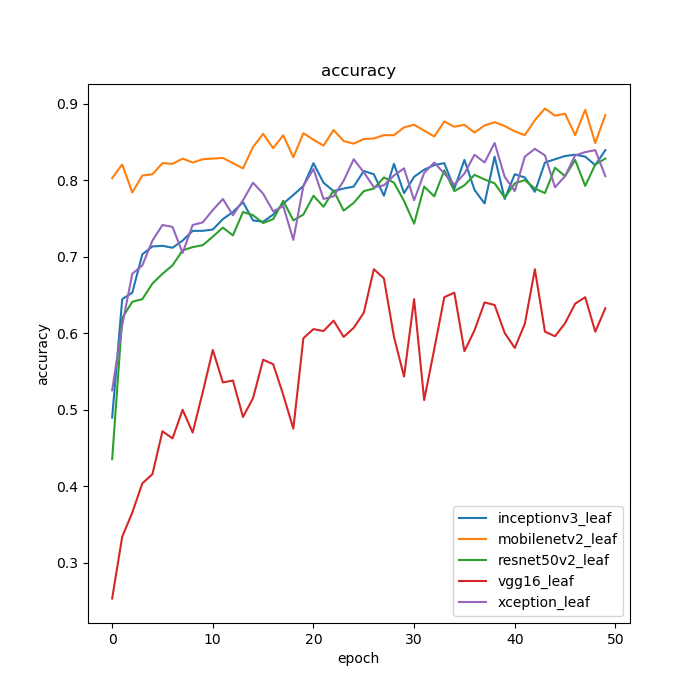
\includegraphics[scale=0.4]{images/leaf_accuracy.png}
			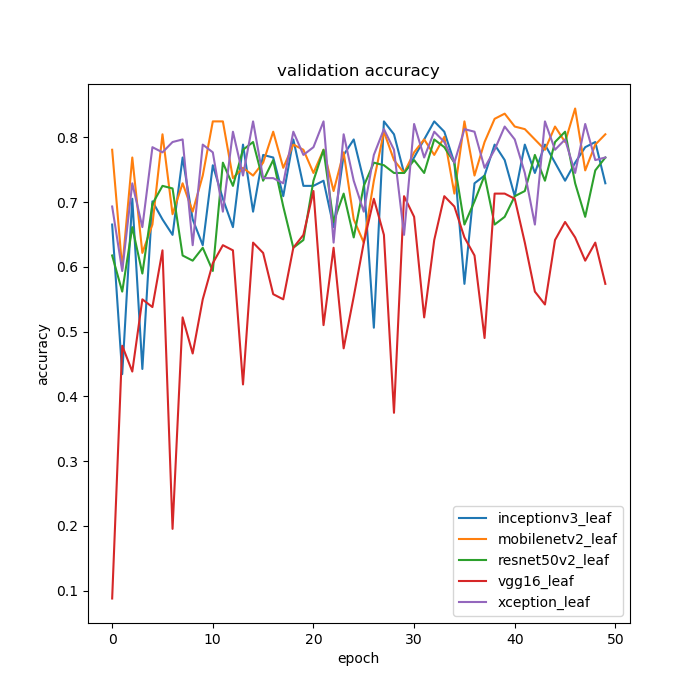
\includegraphics[scale=0.4]{images/leaf_val_accuracy.png}
			\caption{Biểu đồ accuracy trên training set và validation set (gốc)}
		\end{figure}

		\begin{figure}[H]
			\centering
			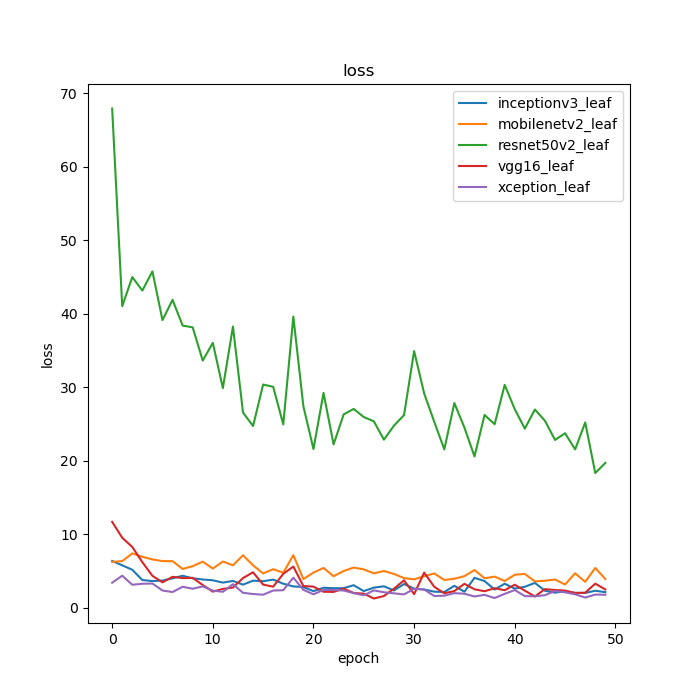
\includegraphics[scale=0.4]{images/leaf_loss.png}
			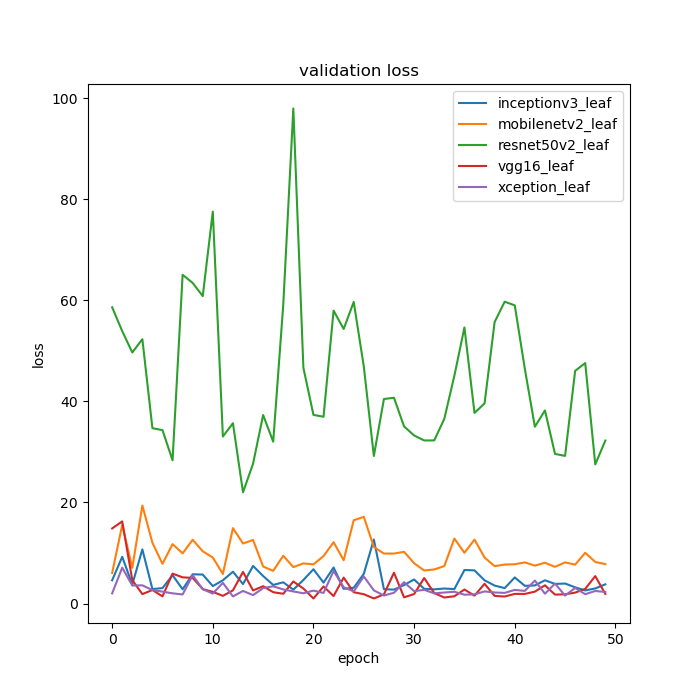
\includegraphics[scale=0.4]{images/leaf_val_loss.png}
			\caption{Biểu đồ loss trên training set và validation set (gốc)}
		\end{figure}
		
		\begin{figure}[H]
			\centering
			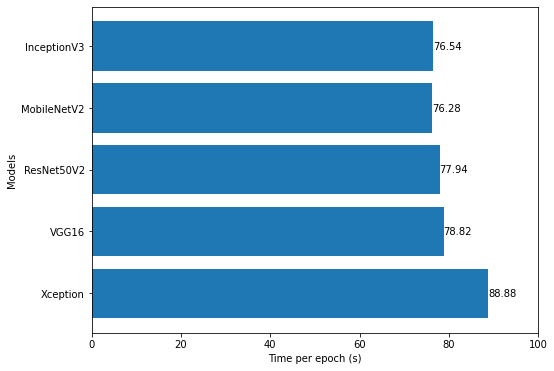
\includegraphics[scale=0.5]{images/original_time}
			\caption{Thời gian trung bình cho mỗi epoch trên dataset (gốc)}
		\end{figure}

		\begin{figure}[H]
			\centering
			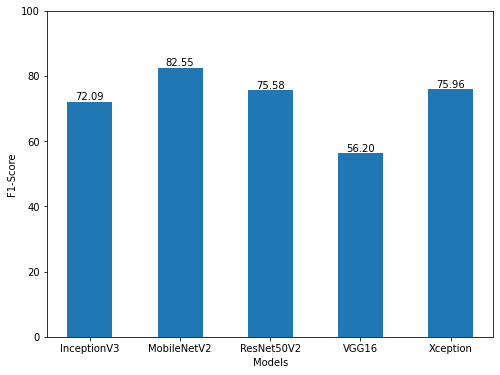
\includegraphics[scale=0.6]{images/original_score}
			\caption{Kết quả đo các model trên test set (gốc)}
		\end{figure}

		MobileNetV2 đạt được F1-score 82.55\%, vượt trội so với các model khác. Tốc độ train của model này cũng nhanh nhất, đạt 76.28s/epoch. Với lợi thế yêu cầu tính toán và yêu cầu bộ nhớ thấp nhờ vào lượng trainable parameter ít hơn đáng kể, MobileNetV2 xử lý khá ổn với input lớn và chưa qua xử lý.

		\begin{figure}[H]
			\centering
			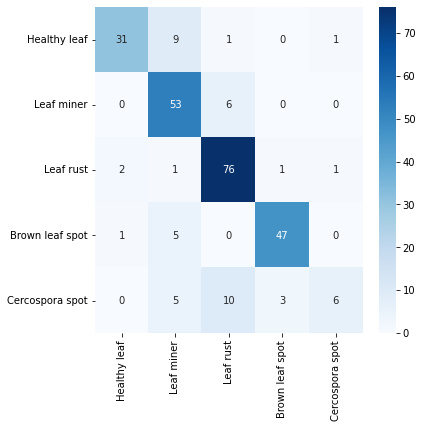
\includegraphics[scale=0.8]{images/mobilenetv2_matrix.png}
			\caption{Confusion Matrix của MobileNetV2 trên test set (gốc)}
		\end{figure}

		Tổng thể, kết quả đo trên dataset gốc của các model không thực sự tốt, khi không có model nào đạt F1-score cao. Việc giữ nguyên ảnh gốc khiến cho khối lượng input rất lớn và không thể train được, trong khi downsample sẽ giảm độ chi tiết, gây khó khăn trong nhận diện. Tốc độ train vẫn còn rất chậm, dù kích thước của input đã giảm.

	\subsubsection{Trên tập dữ liệu đã xử lý}
		\begin{figure}[H]
			\centering
			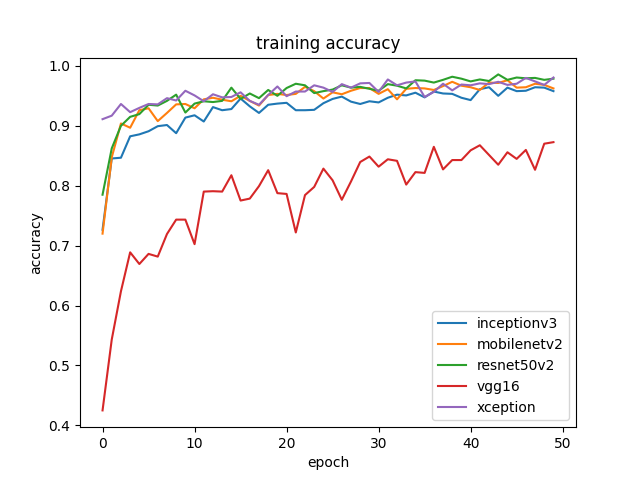
\includegraphics[scale=0.45]{images/accuracy.png}
			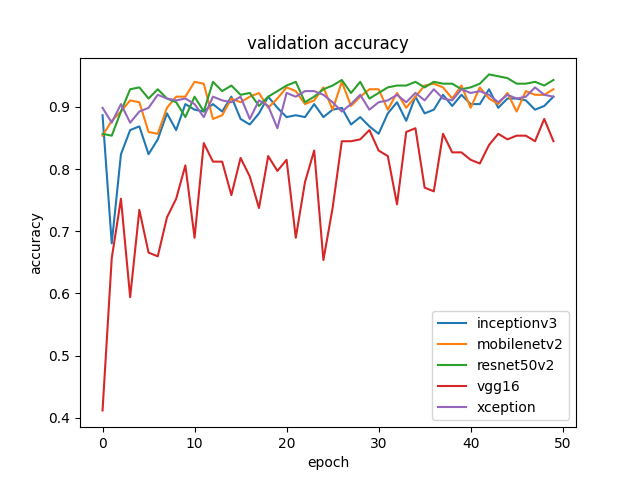
\includegraphics[scale=0.45]{images/val_accuracy.png}
			\caption{Biểu đồ accuracy trên training set và validation set (đã xử lý)}
		\end{figure}

		\begin{figure}[H]
			\centering
			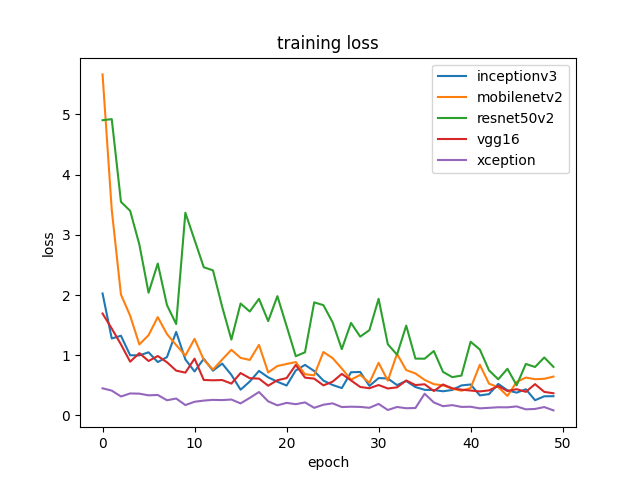
\includegraphics[scale=0.45]{images/loss.png}
			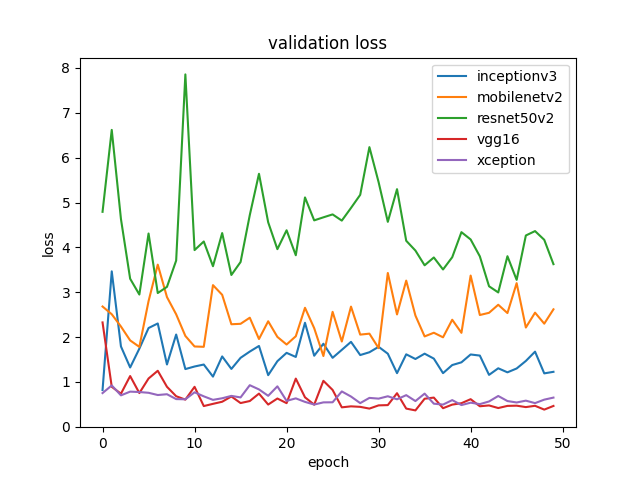
\includegraphics[scale=0.45]{images/val_loss.png}
			\caption{Biểu đồ loss trên training set và validation set (đã xử lý)}
		\end{figure}
		\begin{figure}[H]
			\centering
			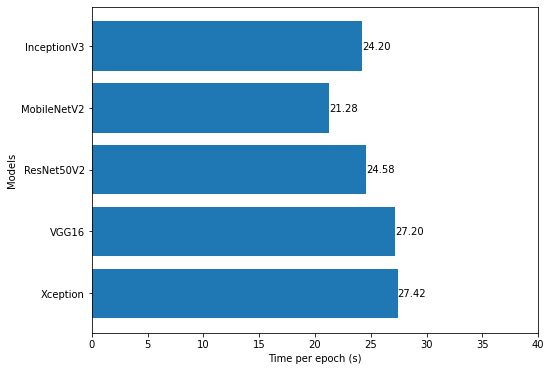
\includegraphics[scale=0.5]{images/processed_time}
			\caption{Thời gian trung bình cho mỗi epoch trên dataset (đã xử lý)}
		\end{figure}
		
		\begin{figure}[H]
			\centering
			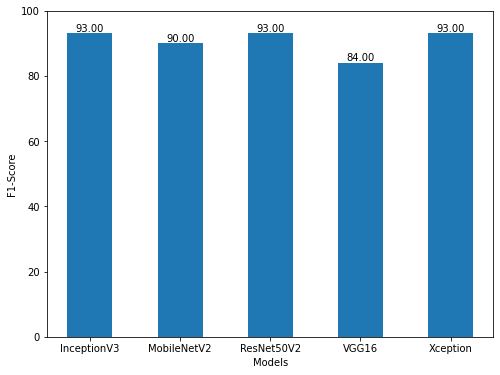
\includegraphics[scale=0.6]{images/processed_score}
			\caption{Kết quả đo các model trên test set (đã xử lý)}
		\end{figure}
		
		Trên dataset đã xử lý, khả năng tính toán của các model có phần khác biệt so với trên dataset gốc. Các kết quả đo đều có sự cải thiện rõ rệt một cách đáng kể.

		Ba model InceptionV3, ResNet50V2 và Xception đều có F1-score đạt 93\%, tốt hơn MobileNetV2 (90\%) và VGG16 (84\%). Cả ba model đều có số lượng parameter và số layer tương đối tương đồng.
		
		MobileNetV2 vẫn là model có tốc độ train nhanh nhất, dù hiệu năng có phần thua thiệt hơn. Sức mạnh của VGG16 kém xa các model còn lại, trong khi thời gian train chỉ nhanh hơn Xception.

		Mặc dù thời gian train chậm nhất, nhưng với lợi thế là model có nhiều tầng nhất, Xception có phần nhỉnh hơn khi chỉ mất vài epoch để các thông số đạt trạng thái gần tối ưu. Xuyên suốt quá trình train, biểu đồ của Xception cũng ổn định hơn nhiều.

		\begin{figure}[H]
			\centering
			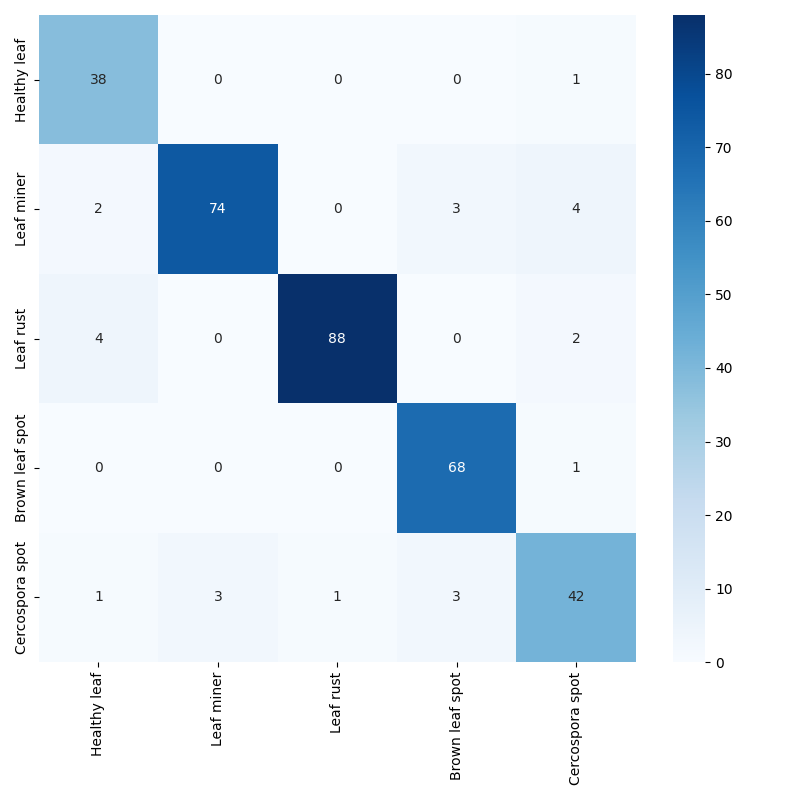
\includegraphics[scale=0.8]{images/xception_matrix.png}
			\caption{Confusion Matrix của Xception trên test set (đã xử lý)}
		\end{figure}

		\subsubsection{Kết luận về mô hình}

		Trên dataset gốc, kết quả thu thập được không quá tốt khi chỉ MobileNetV2 đạt F1-score trên 80\%. Vì vậy, việc xử lý data trước khi train là cần thiết. Kết quả train trên dataset đã xử lý khả quan hơn hoàn toàn. Ba model InceptionV3, ResNet50V2 và Xception thể hiện tương đồng trên dataset này. InceptionV3 có tốc độ train nhanh nhất, còn Xception đạt trạng thái tối ưu sớm nhất.

		Sau quá trình nghiên cứu và thử nghiệm, \textbf{Xception} là model phù hợp nhất với bài toán và phương pháp xử lý dữ liệu.

	\subsection{Ứng dụng}
	Để ứng dụng kết quả từ model trên vào thực tế, một hệ thống gồm mobile app và server, liên lạc qua API để xử lý đã được phát triển.

	\begin{figure}[H]
		\centering
		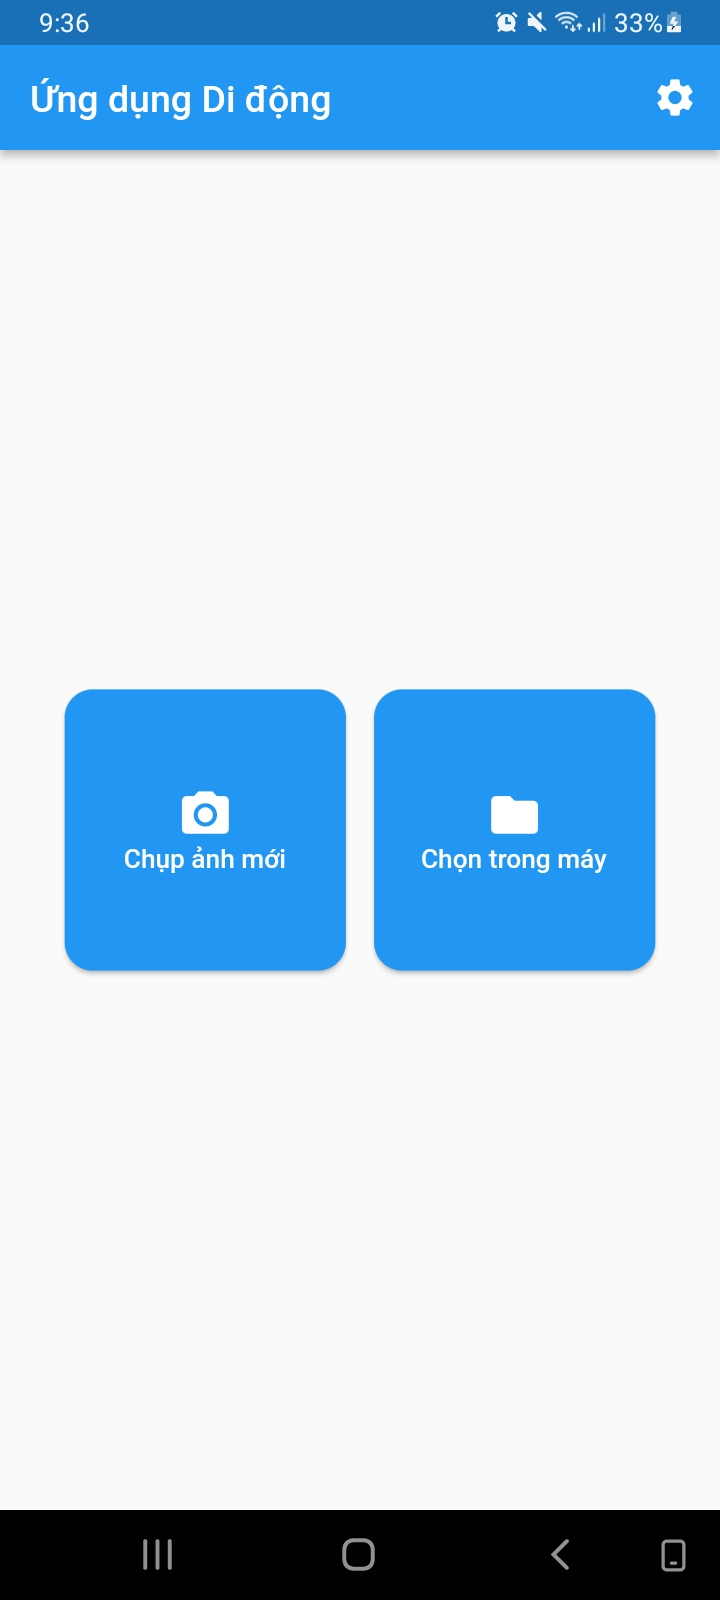
\includegraphics[scale=0.1]{images/screenshot1.jpg}
		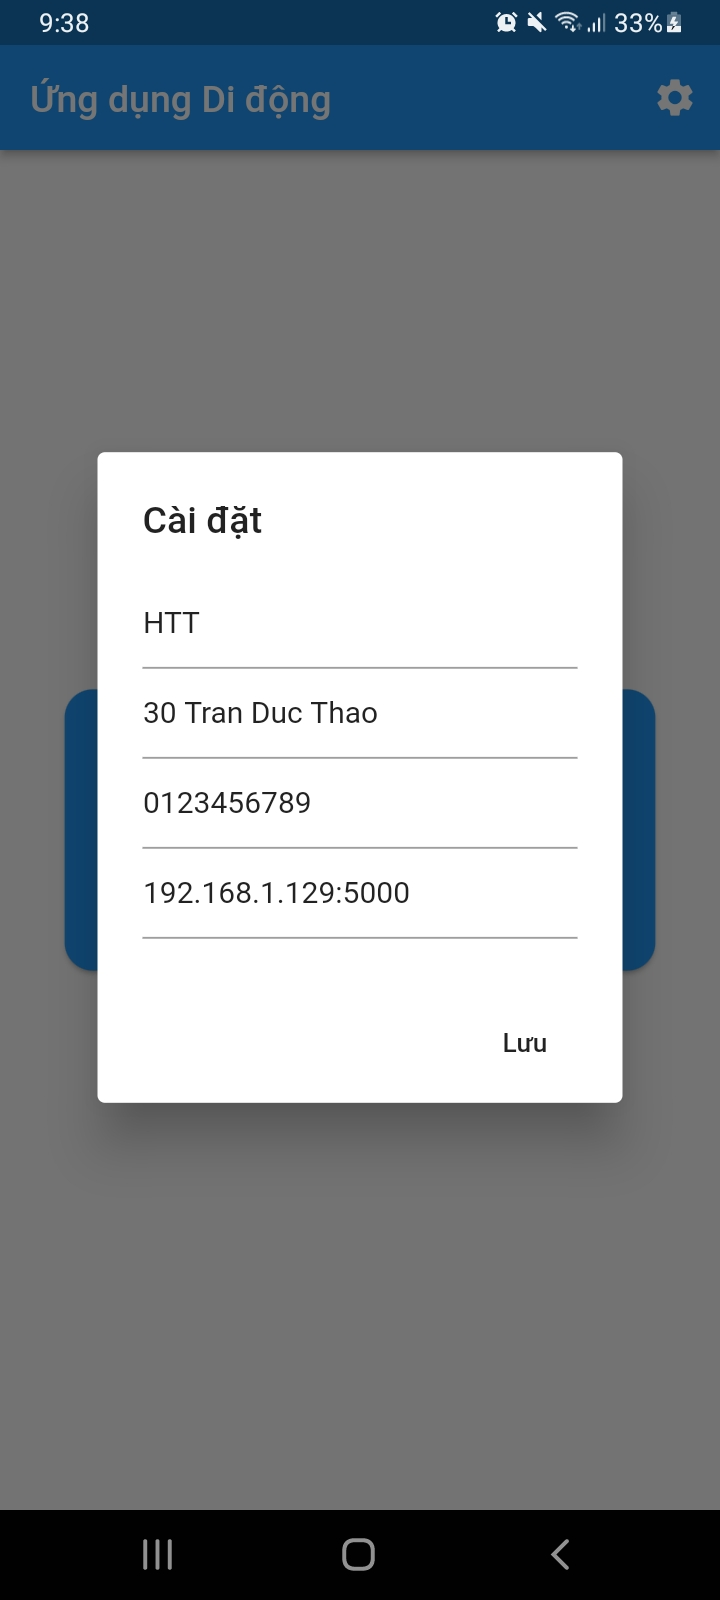
\includegraphics[scale=0.1]{images/screenshot2.jpg}
		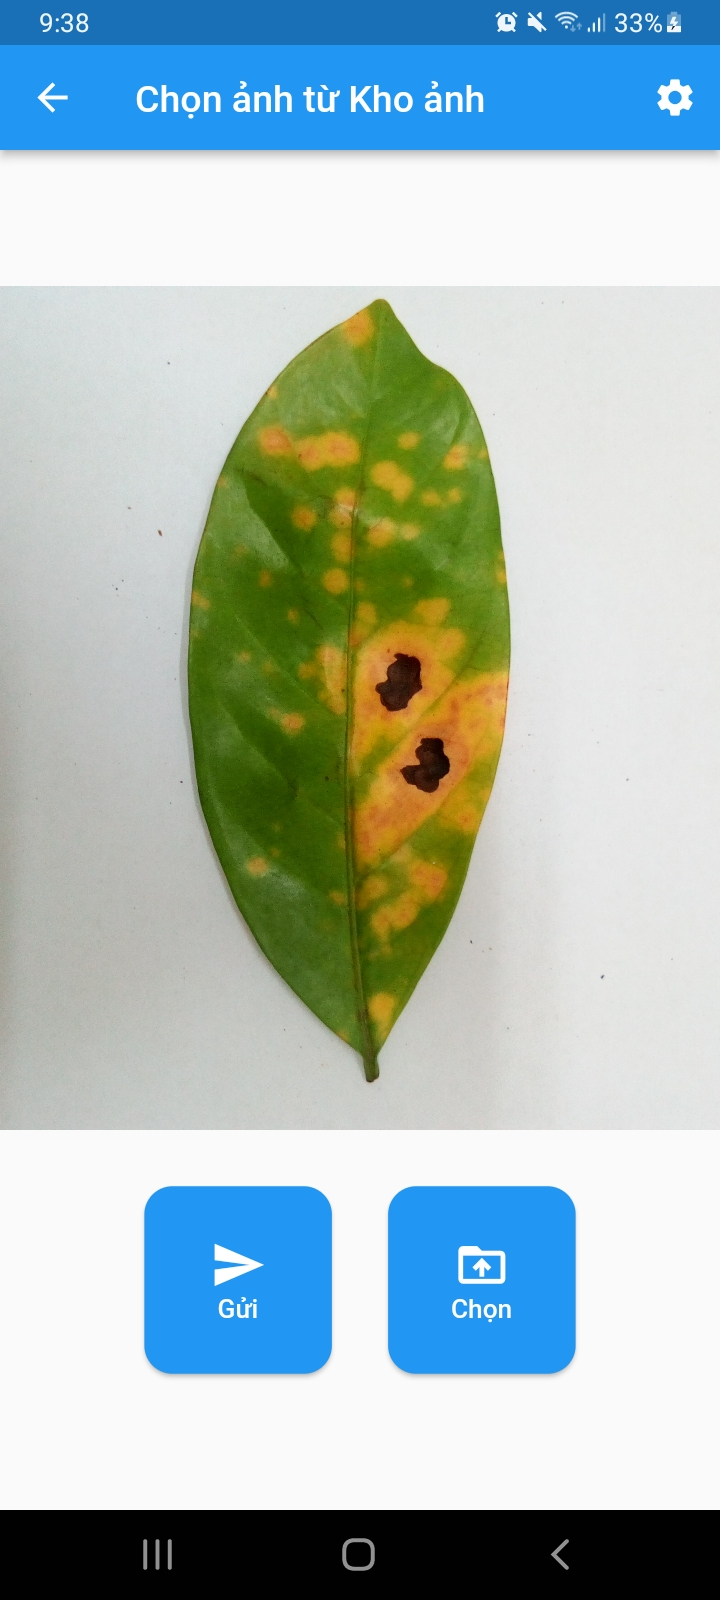
\includegraphics[scale=0.1]{images/screenshot3.jpg}
		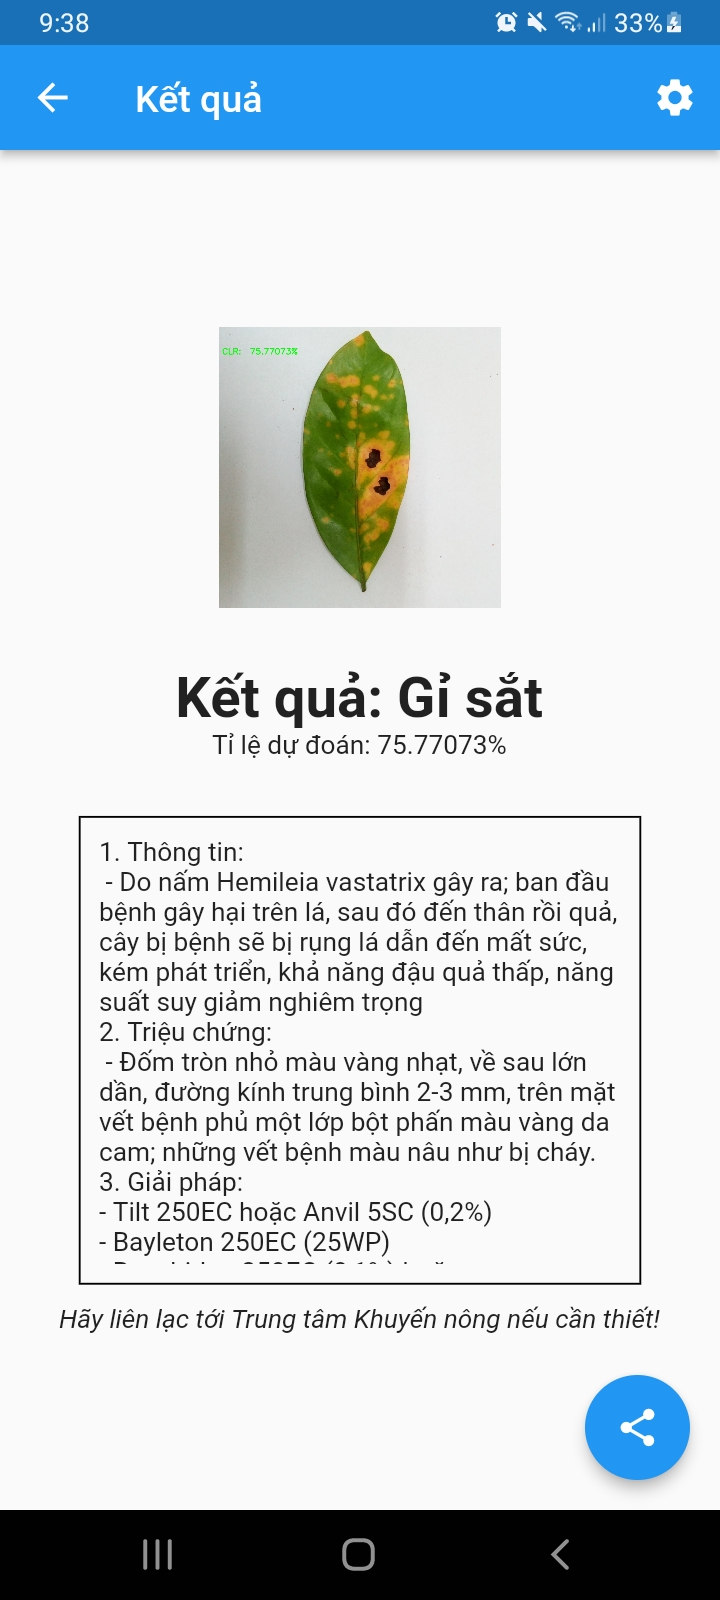
\includegraphics[scale=0.1]{images/screenshot4.jpg}
		\caption{Giao diện của mobile app}
	\end{figure}

	App được xây dựng bằng Flutter, hoạt động được trên cả Android và iOS, có thiết kế đơn giản, dễ sử dụng với bà con, đặc biệt là đồng bào dân tộc thiểu số. API được xây dựng bằng Flask, một web framework gọn nhẹ bằng Python, giúp việc xây dựng nhanh chóng và kết nối thuận tiện tới backend.

	App cho phép người dùng gửi hình ảnh (ảnh có sẵn trong máy hoặc ảnh chụp mới) lên server. Server tiếp nhận, xử lý ảnh bằng model được xây dựng, rồi trả kết quả chẩn đoán về lại app. Các kết quả trả về bao gồm: tên bệnh, một số triệu chứng, đặc điểm đặc trưng và tên một vài thuốc đặc trị cho sâu bệnh. App còn cho phép người dùng chia sẻ thông tin về loại sâu bệnh tìm được qua email hay các trang nhắn tin trên mạng để yêu cầu chuyên gia giúp đỡ thêm.

\section{Đánh giá chung}
	Đề tài này nghiên cứu việc ứng dụng Deep Learning vào việc nhận diện một số sâu bệnh thường gặp, thông qua biểu hiện của lá. Dữ liệu cho việc huấn luyện được thu thập từ khu vực bản địa của tác giả, song song với tìm kiếm trên mạng. Qua thử nghiệm, việc xử lý dữ liệu là cần thiết để tăng cường và cân bằng dữ liệu, giảm khối lượng tính toán mà vẫn đảm bảo khả năng nhận diện. Một số CNN đã được thử nghiệm, trong đó Xception mang lại kết quả tốt nhất trên dataset đã xử lý. Để ứng dụng model vào thực tế, một hệ thống gồm server và mobile app đơn giản đã được xây dựng, có chức năng gửi và tiếp nhận thông tin, đưa đến model để xử lý.
	
	\textbf{Deep Learning là một phương pháp khả thi} để nhận diện sâu bệnh qua hình thái của lá cà phê, và hoàn toàn có thể tiếp tục phát triển trong tương lai, mở rộng sang nhiều giống cây trồng khác, phục vụ người nông dân ở khắp mọi miền đất nước.

	\subsection{Ưu điểm}
	\begin{itemize}
		\item Khả năng nhận diện tương đối chính xác, tỉ lệ thuận với lượng dữ liệu theo thời gian;
		\item Tiết kiệm thời gian, công sức, chi phí cho việc chẩn đoán so với các phương pháp hiện có;
		\item Mobile app gọn nhẹ, đơn giản, dễ sử dụng.
	\end{itemize}

	\subsection{Nhược điểm}
	\begin{itemize}
		\item Tốc độ nhận diện còn chậm, cần một server trung gian đủ mạnh để xử lý;
		\item Dataset còn hạn chế về kích thước và chưa cân bằng giữa các loại sâu bệnh, cần được mở rộng và làm phong phú thêm;
		\item Cơ sở dữ liệu và thông tin chung về các loại sâu bệnh còn ít;
		\item Server chưa thể xử lý thông tin từ nhiều người dùng.
	\end{itemize}

	\subsection{Hướng phát triển}
	\begin{itemize}
		\item Thu thập thêm dữ liệu, khai thác thêm các kỹ thuật tiền xử lý dữ liệu nâng cao hơn, xây dựng một bộ cơ sở dữ liệu trung tâm;
		\item Cải tiến model, cải tiến phương pháp luyện để khai thác hết tiềm năng của model, thử nghiệm với những model mới;
		\item Hoàn thiện, phát triển thêm API cho server và mobile app;
		\item Hợp tác với các nhà nghiên cứu về cây cà phê để tiếp tục hoàn thiện dự án.
	\end{itemize}

\section{Kết luận}
Mục đích nghiên cứu của dự án xuất phát từ tình hình thực tiễn tại chính địa phương nơi tác giả đang học tập và sinh sống; với hy vọng đề tài sẽ góp phần cải thiện ngành trồng trọt cà phê ở Kon Tum, giúp người dân, đặc biệt là đồng bào dân tộc thiểu số vươn lên thoát nghèo, làm giàu chính đáng trên quê hương của mình; góp phần phát triển kinh tế của địa phương.

\section{Dữ liệu và chương trình}
Dữ liệu và chương trình của dự án được tác giả đưa lên các địa chỉ:

\begin{itemize}
	\item Mobile app: \url{https://github.com/jalsol/client}.
	\item Server: \url{https://github.com/jalsol/server}.
\end{itemize}

\section{Tài liệu tham khảo}
[1] Suhartono, Derwin \& Aditya, Wahyu \& Lestari, Miranty \& Yasin,\\Muhammad. (2013). Expert System in Detecting Coffee Plant Diseases. International Journal of Electrical Energy. 156-162. 10.12720/ijoee.1.3.156-162.

[2] M. Kumar, P. Gupta, P. Madhav and Sachin, "Disease Detection in Coffee Plants Using Convolutional Neural Network," 2020 5th International Conference on Communication and Electronics Systems (ICCES), 2020, pp. 755-760, doi: 10.1109/ICCES48766.2020.9138000.

[3] Esgario, J. G., Krohling, R. A., \& Ventura, J. A. (2020) "Deep learning for classification and severity estimation of coffee leaf biotic stress" Computers and Electronics in Agriculture 169, 105162,\\doi:10.1016/j.compag.2019.105162

[4] Krohling, Renato; Esgario, José; Ventura, Jose A. (2019), "BRACOL\\- A Brazilian Arabica Coffee Leaf images dataset to identification and quantification of coffee diseases and pests", Mendeley Data, V1, doi: 10.17632/yy2k5y\\8mxg.1

[5] François Chollet, "Xception: Deep Learning with Depthwise Separable Convolutions", arXiv:1610.02357v3 [cs.CV], Apr 2017.

\end{document}
